         \chapter{The particles that substances are made of}\fancyfoot[LO,RE]{Chemistry: Matter and materials}
\label{chap:composition}
    \setcounter{figure}{1}
    \setcounter{subfigure}{1}
    \label{m38120}
\section{Atoms and compounds}
    \subsection*{The atom as the building block of matter}
            \nopagebreak
            \label{m38120*cid2} $ \hspace{-5pt}\begin{array}{cccccccccccc}   \end{array} $ \hspace{2 pt}\raisebox{-5 pt}{
\includegraphics[width=0.5cm]{col11305.imgs/summary_www.png}} {(section shortcode: P10053 )} \par 
      \label{m38120*id307092}We have now seen that different materials have 
different properties. Some materials are metals and some are non-metals; some 
are electrical or thermal conductors, while others are not. Depending on the 
properties of these materials, they can be used in lots of useful applications. 
But what is it exactly that makes up these materials? In other words, if we were 
to break down a material into the parts that make it up, what would we find? And 
how is it that a material's microscopic structure (the small parts that make up 
the material) is able to give it all these different properties?\par 
      \label{m38120*id307099}The answer lies in the smallest building block of 
matter: the \textbf{atom}. It is the \textsl{type} of atoms, and the way in which they are 
\textsl{arranged} in a material, that affects the 
properties of that substance. This is similar to building materials. We can use bricks, steel, cement, wood, straw (thatch), mud and many other things to build structures from. In the same way that the choice of building material affects the properties of the structure, so the atoms that make up matter affect the properties of matter.\par 
      \label{m38120*id307459}It is not often that substances are found in atomic 
form (just as you seldom find a building or structure made from one building material). Normally, atoms are bonded (joined) to other atoms to form \textbf{compounds} or \textbf{molecules}. It is only in the \textsl{noble gases} (e.g. helium, neon and argon) that atoms 
are found individually and are not bonded to other atoms. We looked at some of the 
reasons for this in earlier chapters.\par 
    \section*{Compounds}
            \nopagebreak
            \label{m38120*cid3} $ \hspace{-5pt}\begin{array}{cccccccccccc}   \end{array} $ \hspace{2 pt}\raisebox{-5 pt}{
\includegraphics[width=0.5cm]{col11305.imgs/summary_www.png}} {(section shortcode: P10054 )} \par 
\par
            \label{m38120*fhsst!!!underscore!!!id74}
\Definition{   \label{id2456442}\textbf{ Compound }} { \label{m38120*meaningfhsst!!!underscore!!!id74}
      A compound is a group of two or more different atoms that are 
attracted to each other by relatively strong forces or bonds. 
       } 
      \label{m38120*id307508}Almost everything around us is made up of molecules. The only substances that are not made of molecules, but instead are individual atoms are the noble gases.
\textsl{Water} is made up of molecules, each of 
which has two hydrogen atoms joined to one oxygen atom. \textsl{Oxygen} is a molecule that is made up of two oxygen 
atoms that are joined to one another. Even the food that we eat is made up of 
molecules that contain atoms of elements such as carbon, hydrogen and oxygen 
that are joined to one another in different ways. All of these are known as 
\textbf{small molecules} because there are only a few 
atoms in each molecule. \textbf{Giant molecules} are 
those where there may be millions of atoms per molecule. Examples of giant 
molecules are \textsl{diamonds}, which are made up 
of millions of carbon atoms bonded to each other and \textsl{metals}, which are made up of millions of metal atoms 
bonded to each other.\par 
\subsection*{Covalent bonding}
      \label{m38120*eip-819}As we learnt in Chemical bonding atoms can share electrons to form covalent bonds or exchange electrons to form ionic bonds. Covalently bonded substances are known as molecular compounds. Ionically bonded substances are known as ionic compounds. We also learnt about metallic bonding. In a metal the atoms lose their outermost electrons to form positively charged ions that are arranged in a lattice, while the outermost electrons are free to move amongst the spaces of the lattice. \par \label{m38120*eip-394}We can classify covalent molecules into covalent molecular structures and covalent network structures. Covalent molecular structures are simply individual covalent molecules and include water, oxygen, sulphur (${\mathrm{S}}_{8}$) and buckminsterfullerene (${\mathrm{C}}_{60}$). All covalent molecular structures are simple molecules. Covalent network structures are giant lattices of covalently bonded molecules, similar to the ionic lattice. Examples include diamond, graphite and silica (${\mathrm{SiO}}_{2}$). All covalent network structures are giant molecules.\par 
\subsection*{Ionic compounds and metals}
\label{m38120*eip-860}Examples of ionic substances are sodium chloride ($\mathrm{NaCl}$) and potassium permanganate (${\mathrm{KMnO}}_{4}$). Examples of metals are copper, zinc, titanium, gold, etc.\par \label{m38120*uid1}
            \subsection*{Representing molecules}
            \nopagebreak
        \label{m38120*id307557}The structure of a molecule can be shown in many 
different ways. Sometimes it is easiest to show what a molecule looks like by 
using different types of \textbf{diagrams}, but at 
other times, we may decide to simply represent a molecule using its \textbf{chemical formula} or its written name.\par 
        \label{m38120*id307573}\begin{enumerate}[noitemsep, label=\textbf{\arabic*}. ] 
            \label{m38120*uid2}\item \textbf{Using formulae to show the structure of a 
molecule.}
A \textbf{chemical formula} is an abbreviated 
(shortened) way of describing a molecule, or some other chemical substance. In 
the chapter on classification of matter, we saw how chemical compounds can be 
represented using element symbols from the Periodic Table. A chemical formula 
can also tell us the \textsl{number} of atoms of 
each element that are in a molecule and their \textsl{ratio} in that molecule.
For example, the chemical formula for a molecule of carbon dioxide is
${\mathrm{CO}}_{2}$
The formula above is called the \textbf{molecular 
formula} of that compound. The formula tells us that in one molecule 
of carbon dioxide, there is one atom of carbon and two atoms of oxygen. The 
ratio of carbon atoms to oxygen atoms is 1:2.
\vspace{\rubberspace}\par
        \label{m38120*fhsst!!!underscore!!!id87}
 \Definition{   \label{id2456697}\textbf{ Molecular formula }} { \label{m38120*meaningfhsst!!!underscore!!!id87}
This is a concise way of expressing information about the atoms that make up a 
particular chemical compound. The molecular formula gives the exact number of 
each type of atom in the molecule. 
 } 

A molecule of glucose has the molecular formula:
${\mathrm{C}}_{6}{\mathrm{H}}_{12}{\mathrm{O}}_{6}$.
In each glucose molecule, there are six carbon atoms, twelve hydrogen atoms and 
six oxygen atoms. The ratio of carbon:hydrogen:oxygen is 6:12:6. We can simplify 
this ratio to write 1:2:1, or if we were to use the element symbols, the formula 
would be written as ${\mathrm{CH}}_{2}\mathrm{O}$. This is called the \textbf{empirical formula} of the molecule.
\vspace{\rubberspace}\par
        \label{m38120*fhsst!!!underscore!!!id93}
\Definition{   \label{id2456770}\textbf{ Empirical formula }} { \label{m38120*meaningfhsst!!!underscore!!!id93}
This is a way of expressing the \textsl{relative} 
number of each type of atom in a chemical compound. In most cases, the empirical 
formula does not show the exact number of atoms, but rather the simplest 
\textsl{ratio} of the atoms in the compound. 
 } 

The empirical formula is useful when we want to write the 
formula for a \textsl{giant molecule}. Since giant 
molecules may consist of millions of atoms, it is impossible to say exactly how 
many atoms are in each molecule. It makes sense then to represent these 
molecules using their empirical formula. So, in the case of a metal such as 
copper, we would simply write Cu, or if we were to represent a molecule of 
sodium chloride, we would simply write NaCl.
Chemical formulae therefore tell us something about the \textsl{types} of atoms that are in a molecule and the 
\textsl{ratio} in which these atoms occur in the 
molecule, but they don't give us any idea of what the molecule actually looks 
like, in other words its \textsl{shape}. To show 
the shape of molecules we can represent molecules using diagrams.
Another type of formula that can be used to describe a molecule is its \textbf{structural formula}. A structural formula uses a 
graphical representation to show a molecule's structure                    
(Figure \ref{fig:representing isobutane}).
    \setcounter{subfigure}{0}
\begin{figure}[h]
\begin{center}
\begin{pspicture}(-5,-1)(5,0.6)
%\psgrid[gridcolor=lightgray]
\rput(-3,0){(a) \textbf{C$_{4}$H$_{10}$}}
\rput(-1,0){(b) \textbf{C$_{2}$H$_{5}$}}
\rput(1,0){(c) \chemfig{CH(-[2]CH_3)(-[7]CH_3)(-[5]CH_3)}}
\end{pspicture}
\caption{Diagram showing (a) the molecular, (b) the empirical and (c) the structural formula of isobutane}
\label{fig:representing isobutane}
\end{center}
\end{figure}      
\label{m38120*uid4}\item \textbf{Using diagrams to show the 
structure of a molecule}
Diagrams of molecules are very useful because they help us to picture how the 
atoms are arranged in the molecule and they help us to see the shape of the 
molecule. There are two types of diagrams that are commonly used:
\label{m38120*id307860}\begin{itemize}[noitemsep]
            \label{m38120*uid5}\item 
\textsl{Ball and stick models}
This is a 3-dimensional molecular model that uses 'balls' to represent atoms and 
'sticks' to represent the bonds between them. The centres of the atoms (the 
balls) are connected by straight lines which represent the bonds between them. A 
simplified example is shown in Figure~11.2.
    \setcounter{subfigure}{0}
\begin{figure}[h]
\begin{center}
\begin{pspicture}(-3,-1)(3,2)
%\psgrid[gridcolor=lightgray]
\rput(-1,0){
\psellipse(0,1.5)(0.5,0.5)
\psline{->}(0.5,1.5)(1.5,1.5)
\rput(2.95,1.5){oxygen atom}
\psellipse(-2.1,0.2)(0.3,0.3)
\psellipse(0.8,-0.6)(0.3,0.3)
\psline{->}(1.1,-0.6)(1.5,-0.6)
\rput(3,-0.6){hydrogen atom}
\psline(-0.4,1.3)(-1.8,0.25)
\psline(0.3,1.1)(0.8,-0.35)
}
\end{pspicture}
\caption{A ball and stick model of a water molecule}
\label{fig:water ball and stick}
\end{center}
\end{figure}
       \label{m38120*uid7}\item \textsl{Space-filling model}
This is also a 3-dimensional molecular model. The atoms are represented by 
spheres.
Figure~11.3 and Figure~11.4 are some examples of 
\textbf{simple molecules} that are represented in 
different ways. \\
\begin{minipage}{.5\textwidth}
%     \setcounter{subfigure}{0}
% \begin{figure}[h]
\begin{center}
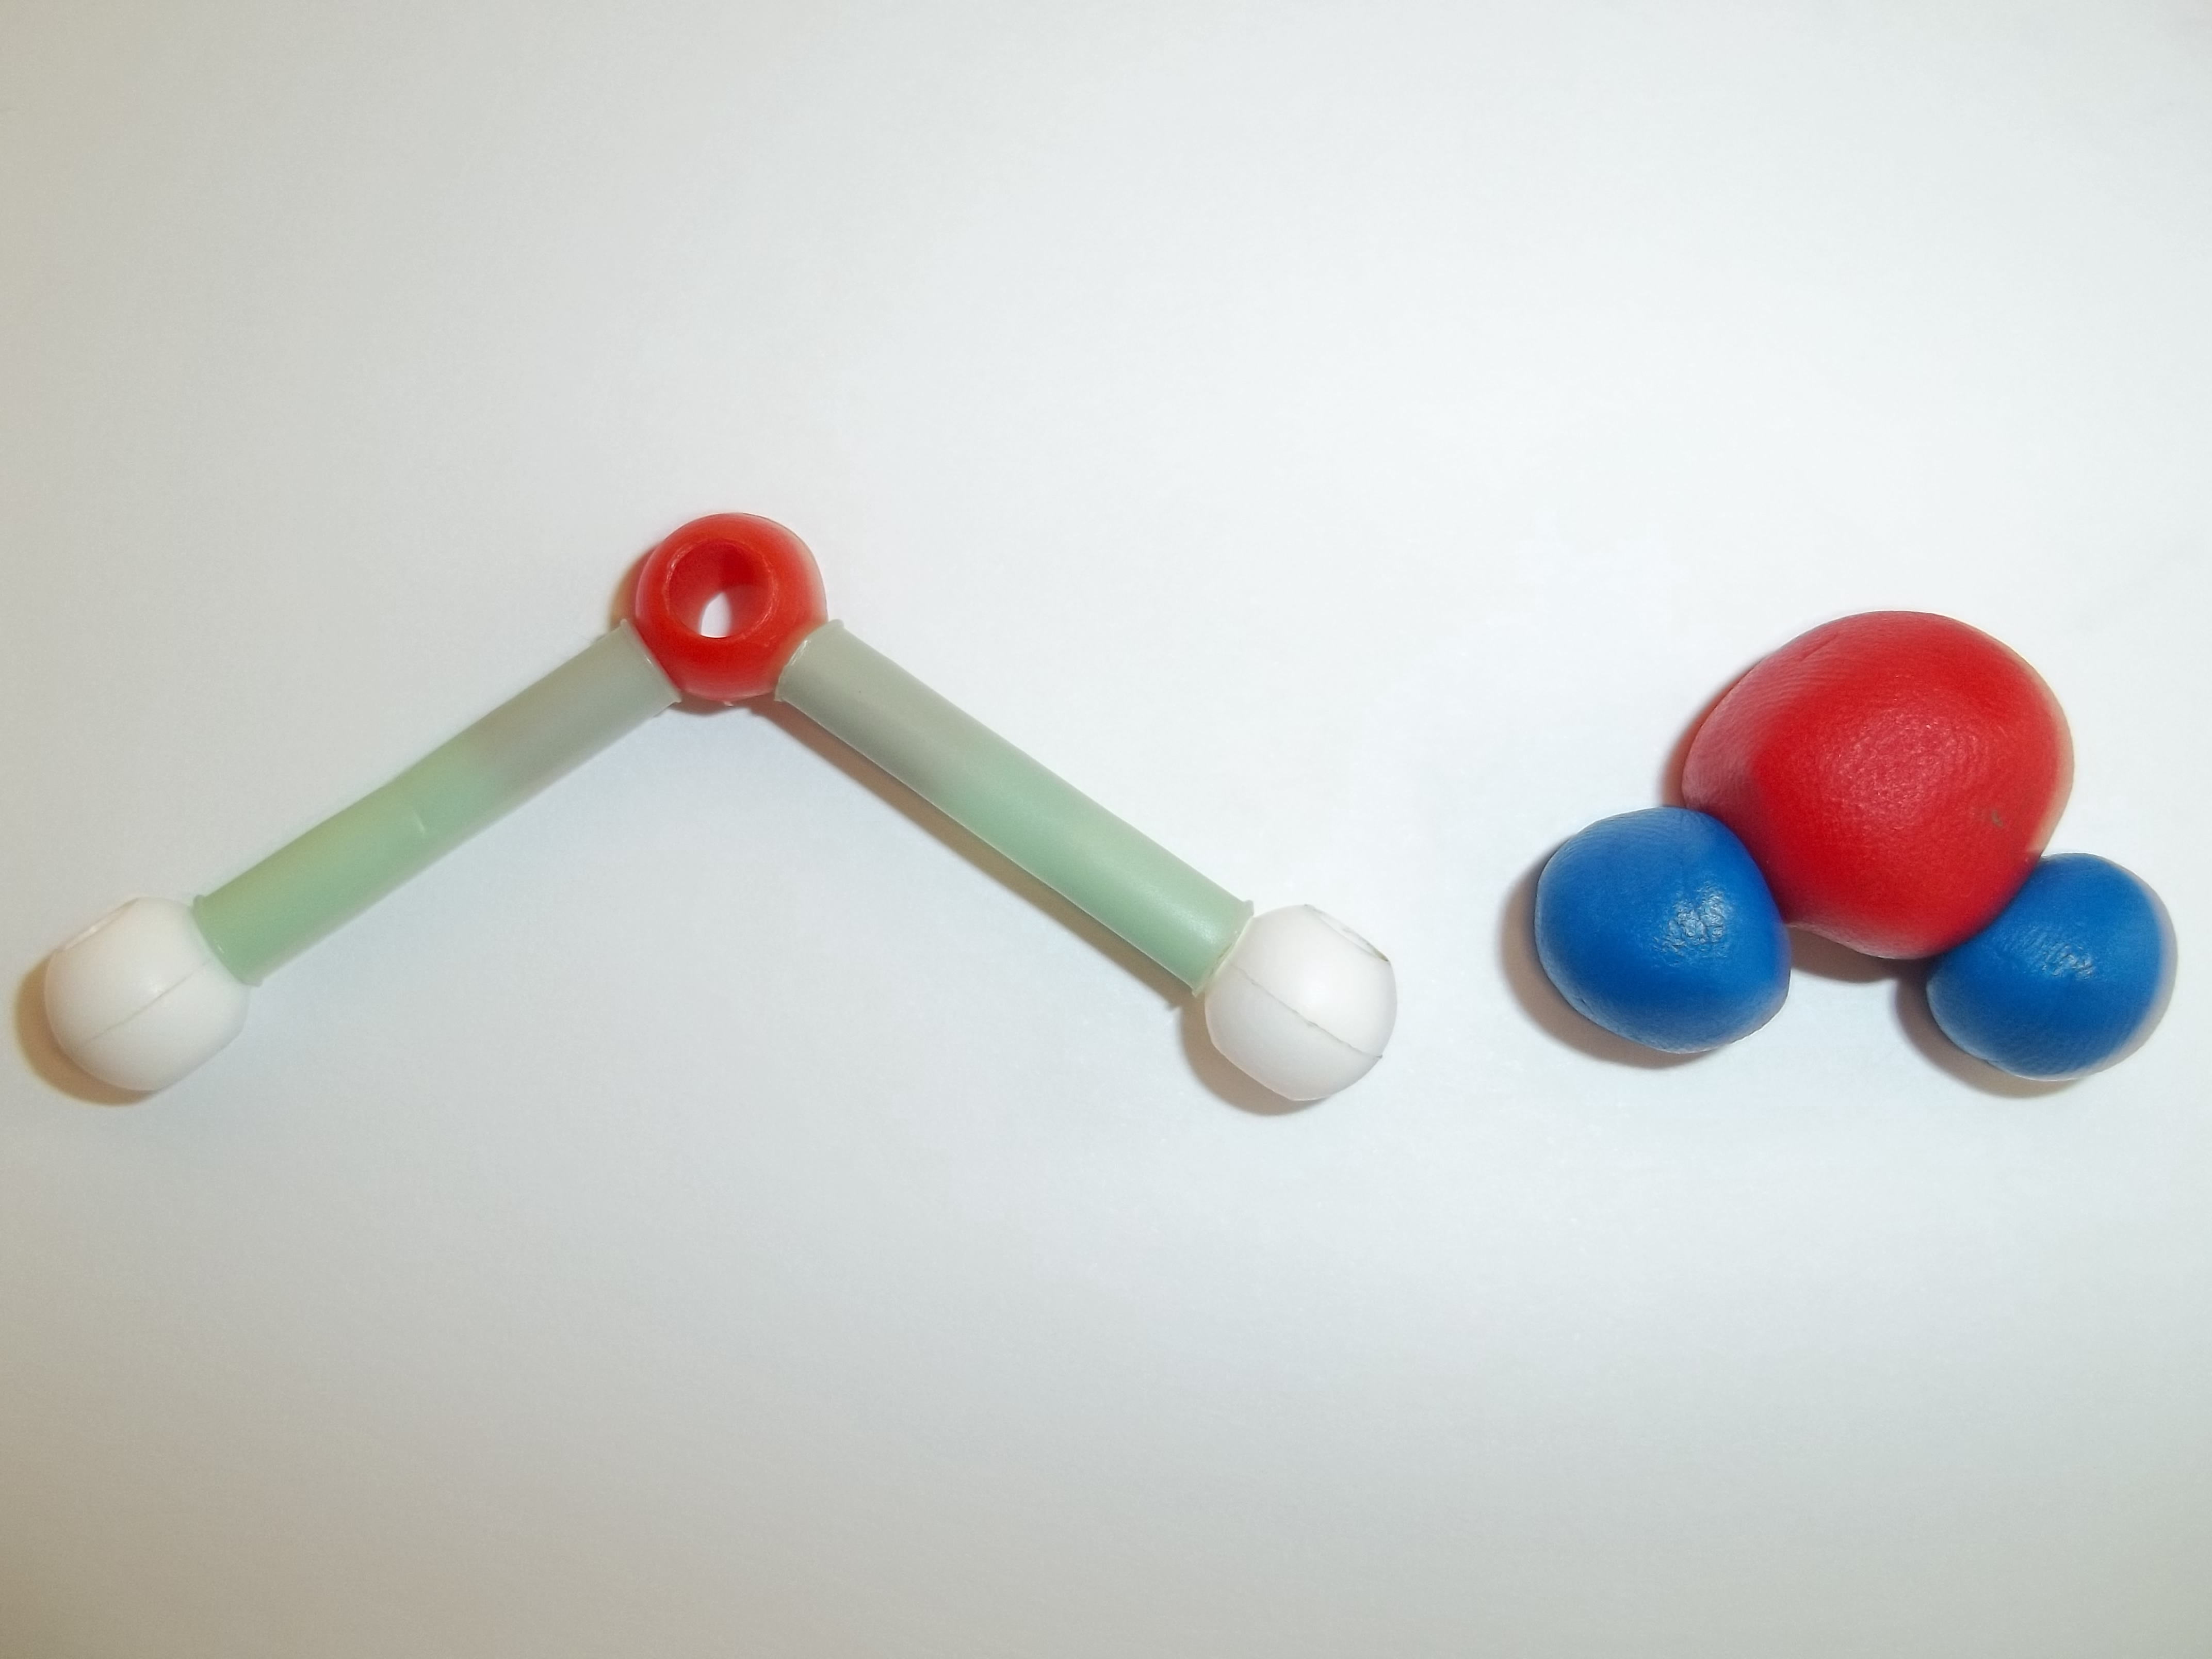
\includegraphics[width=0.8\textwidth]{photos/water.jpg}
% \caption{A space-filling model and structural formula of a water molecule. Each molecule is made up of two hydrogen atoms that are attached to one oxygen atom. This is a simple molecule.}
% \label{fig:microscopic:water molecule}
\end{center}
% \end{figure}    
\end{minipage}
\begin{minipage}{.5\textwidth}
%     \setcounter{subfigure}{0}
% \begin{figure}[h]
\begin{center}
\includegraphics[width=0.8\textwidth]{photos/ammonia.jpg}
% \caption{A space-filling model and structural formula of a molecule of ammonia. Each molecule is made up of one nitrogen atom and three hydrogen atoms. This is a simple molecule.}
% \label{fig:microscopic:ammonia}
\end{center}
% \end{figure}
\end{minipage}
       \end{itemize} \noindent
Figure \ref{fig:microscopic:diamond} shows the bonds between the carbon atoms in diamond, 
which is a \textbf{giant molecule}. Each carbon atom 
is joined to four others, and this pattern repeats itself until a complex 
\textsl{lattice} structure is formed. Each black 
ball in the diagram represents a carbon atom, and each line represents the bond 
between two carbon atoms. Note that the carbon atoms on the edges are actually 
bonded to four carbon atoms, but some of these carbon atoms have been omitted.
    \setcounter{subfigure}{0}
\begin{figure}[h]
\begin{center}
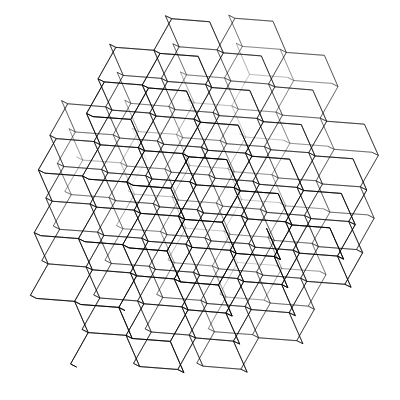
\includegraphics[width=0.3\textwidth]{photos/Diamond_Carbon.png}
\caption{Diagrams showing the microscopic structure of diamond.}
\label{fig:microscopic:diamond}
\end{center}
\end{figure}
       \end{enumerate}
\label{m38120*notfhsst!!!underscore!!!id112}
\Ifact{Diamonds are most often thought of in terms of their use in the 
jewellery industry. However, about 80\% of mined diamonds are unsuitable for use 
as gemstones and are therefore used in industry because of their strength and 
hardness. These properties of diamonds are due to the strong covalent bonds 
(covalent bonding will be explained later) between the carbon atoms in diamond. 
The most common uses for diamonds in industry are in cutting, drilling, 
grinding, and polishing.}

	\par
\label{m38120*uid8310432}This website\footnote{http://alteredqualia.com/canvasmol/}
         allows you to view several molecules. You do 
not need to know these molecules, this is simply to allow you to see one way of 
representing molecules. 
    \setcounter{subfigure}{0}
	\begin{figure}[H] % horizontal\label{m38120*uid10123}
    \begin{center}
    \label{m38120*uid101!!!underscore!!!media}\label{m38120*uid10123!!!underscore!!!printimage}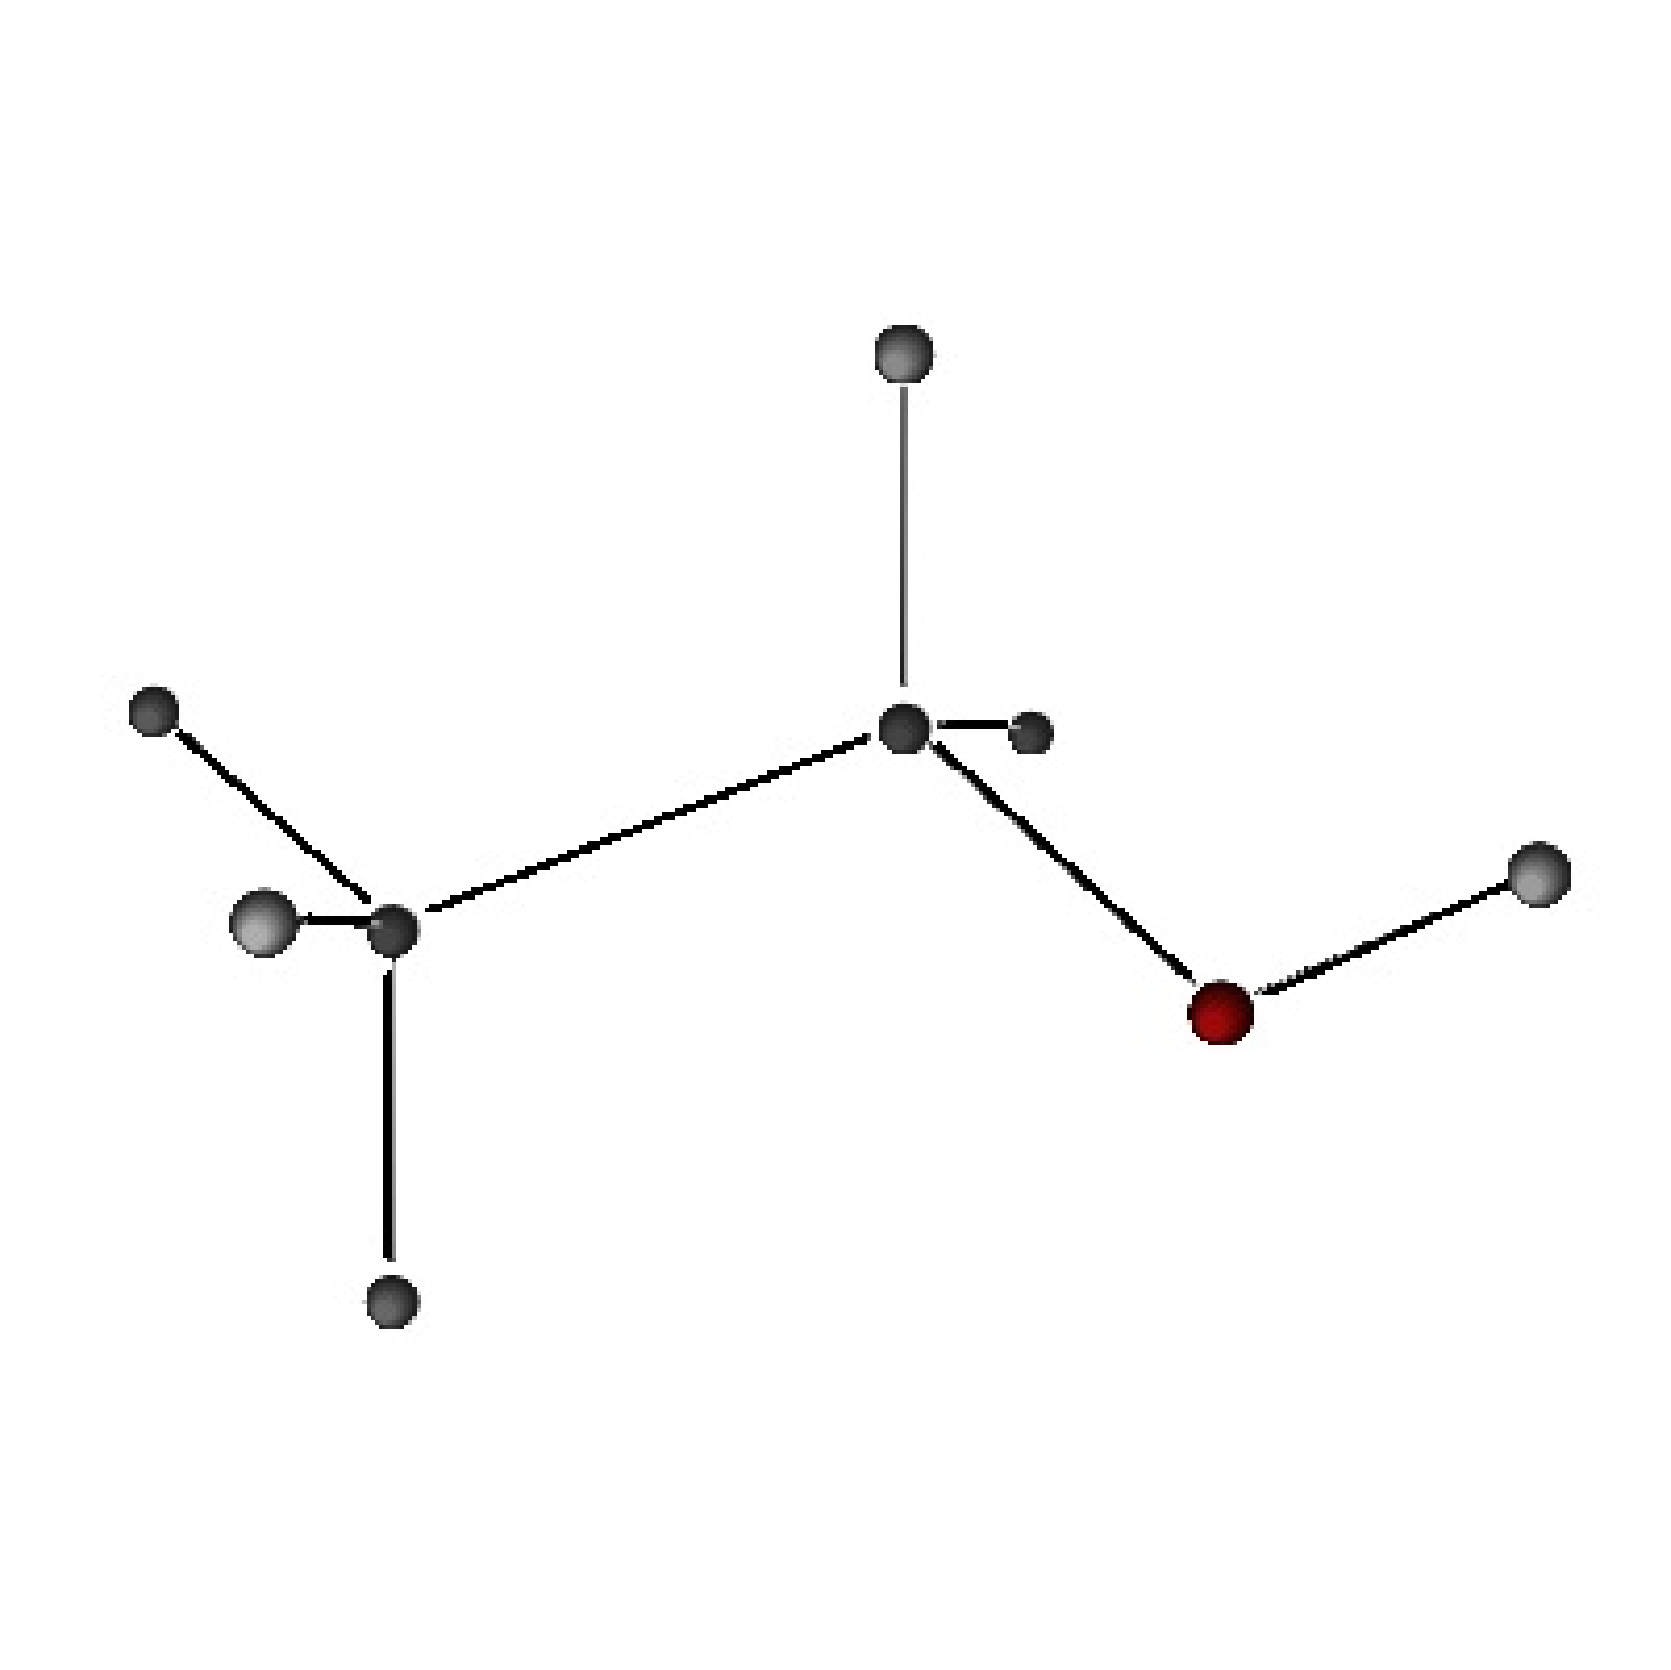
\includegraphics[width=6cm]{col11305.imgs/m38120_canvasmol.png} % m38120;canvasmol.png;;;6.0;8.5;
      \vspace{2pt}
    \vspace{\rubberspace}\par \begin{cnxcaption}
	  \small \textbf{Figure 11.6: }Ball-and-stick view of ethanol from http://alteredqualia.com/canvasmol/\footnotemark{}
	\end{cnxcaption}
    \vspace{.1in}
    \end{center}
 \end{figure}   
    \addtocounter{footnote}{-1}
\par 
\label{m38120*secfhsst!!!underscore!!!id115}
            \begin{exercises}{ Atoms and molecules         }
            \nopagebreak
            \label{m38120*id308039}\begin{enumerate}[noitemsep, label=\textbf{\arabic*}. ] 
            \label{m38120*uid11}\item In each of the following, say whether the chemical 
substance is made up of single atoms, simple molecules or giant molecules.
\label{m38120*id308055}\begin{enumerate}[noitemsep, label=\textbf{\alph*}. ] 
            \label{m38120*uid12}\item ammonia gas (${\mathrm{NH}}_{3}$)
\label{m38120*uid13}\item zinc metal ($\mathrm{Zn}$)
\label{m38120*uid14}\item graphite ($\mathrm{C}$)
\label{m38120*uid15}\item nitric acid (${\mathrm{HNO}}_{3}$)
\label{m38120*uid16}\item neon gas ($\mathrm{He}$)
\end{enumerate}
\label{m38120*uid17}\item Refer to the diagram below and then answer the 
questions that follow:
    \setcounter{subfigure}{0}
	\begin{figure}[H] % horizontal\label{m38120*id308155}
\begin{center}
\begin{pspicture}(-2.6,-2.4)(6,2)
\SpecialCoor
%\psgrid[gridcolor=lightgray]

\psset{unit=0.75}

\pscircle[fillcolor=white,fillstyle=solid](2,0){1.5}
\pscircle[fillcolor=white,fillstyle=solid](0,0){2}
\psarc[fillcolor=white,fillstyle=solid](-2,0){1.5}{45}{-45}
\rput(-2,0){\pscurve(1.5;45)(-1.5;180)(1.5;-45)}

\psset{unit=1.5}
\rput(4,0){\pnode(-1,0){RO}\pnode(0,0){C}\pnode(1,0){LO}
\pnode(-1,0.075){ROO}\pnode(0,0.075){CO}\pnode(1,0.075){LOO}
\psline(RO)(C)
\psline(LO)(C)
\psline(ROO)(CO)
\psline(LOO)(CO)
\rput*(C){C}
\rput*(LO){O}
\rput*(RO){O}}
\end{pspicture}
\end{center}
 \end{figure}       \label{m38120*id308161}\begin{enumerate}[noitemsep, label=\textbf{\alph*}. ] 
            \label{m38120*uid18}\item Identify 
the molecule.
\label{m38120*uid19}\item Write the molecular formula for the molecule.
\label{m38120*uid20}\item Is the molecule a simple or giant molecule?
\end{enumerate}
\label{m38120*uid21}\item Represent each of the following molecules using its 
\textsl{chemical formula}, \textsl{structural formula} and \textsl{ball and stick model}.
\label{m38120*id308228}\begin{enumerate}[noitemsep, label=\textbf{\alph*}. ] 
            \label{m38120*uid22}\item Hydrogen\label{m38120*uid23}\item Ammonia\label{m38120*uid24}\item sulphur dioxide
\end{enumerate}
\end{enumerate}
\par \raisebox{-5 pt}{
\includegraphics[width=0.5cm]{col11305.imgs/summary_www.png}} Find the answers with the shortcodes:
 \par \begin{tabular}[h]{cccccc}
 (1.) li5  &  (2.) liN  &  (3.) liR  & \end{tabular}
\end{exercises}
    \section{ Summary}
            \nopagebreak
            \label{m38120*cid7} $ \hspace{-5pt}\begin{array}{cccccccccccc}   \end{array} $ \hspace{2 pt}\raisebox{-5 pt}{
\includegraphics[width=0.5cm]{col11305.imgs/summary_www.png}} {(section shortcode: P10055 )} \par 
      \label{m38120*id311034}\begin{itemize}[noitemsep]
            \label{m38120*uid67}\item The smallest unit of matter is the \textbf{atom}. Atoms can combine to form \textbf{molecules}.
\label{m38120*uid68}\item A \textbf{compound} is a 
group of two or more atoms that are attracted to each other by chemical bonds.
\label{m38120*uid69}\item A \textbf{small molecule} 
consists of a few atoms per molecule. A \textbf{giant 
molecule} consists of millions of atoms per molecule, for example 
metals and diamonds.
\label{m38120*uid70}\item The structure of a molecule can be represented in a 
number of ways.
\label{m38120*uid71}\item The \textbf{chemical formula} 
of a molecule is an abbreviated way of showing a molecule, using the symbols for 
the elements in the molecule. There are two types of chemical formulae: 
molecular and empirical formula.
\label{m38120*uid72}\item The \textbf{molecular 
formula} of a molecule gives the exact number of atoms of each element 
that are in the molecule.
\label{m38120*uid73}\item The \textbf{empirical 
formula} of a molecule gives the relative number of atoms of each 
element in the molecule.
\label{m38120*uid74}\item Molecules can also be represented using \textbf{diagrams}.
\label{m38120*uid75}\item A \textbf{ball and stick} 
diagram is a 3-dimensional molecular model that uses 'balls' to represent atoms 
and 'sticks' to represent the bonds between them.
\label{m38120*uid76}\item A \textbf{space-filling 
model} is also a 3-dimensional molecular model. The atoms are 
represented by spheres.
\label{m38120*uid77}\item In a molecule, atoms are held together by \textbf{chemical bonds} or \textbf{intramolecular forces}. Covalent bonds, ionic bonds and 
metallic bonds are examples of chemical bonds.
\label{m38120*uid78}\item A \textbf{covalent bond} 
exists between non-metal atoms. An \textbf{ionic bond} 
exists between non-metal and metal atoms and a \textbf{metallic 
bond} exists between metal atoms.
\label{m38120*uid79}\item \textbf{Intermolecular 
forces} are the bonds that hold \textsl{molecules} together.
\end{itemize}
\label{m38120*secfhsst!!!underscore!!!id497}
            \begin{eocexercises}{Composition of matter}
            \nopagebreak
            \label{m38120*id311490}\begin{enumerate}[noitemsep, label=\textbf{\arabic*}. ] 
            \label{m38120*uid87}\item Give one word or term for each of the following 
descriptions.
\label{m38120*id34411506}\begin{enumerate}[noitemsep, label=\textbf{\alph*}. ] 
            \label{m38120*uid90}\item A composition of two or more atoms that act as a unit.
\label{m38120*uid9221}\item Chemical formula that gives the relative number of atoms 
of each element that are in a molecule.
\end{enumerate}
\label{m38120*uid227}\item Give a definition for each of the following terms: 
descriptions.
\label{m38120*id311506}\begin{enumerate}[noitemsep, label=\textbf{\alph*}. ] 
            \label{m38120*uid930}\item molecule
\label{m38120*uid91}\item Ionic compound
\item Covalent network structure\item Empirical formula\item Ball-and-stick model\end{enumerate}
\label{m38120*uid92}\item Ammonia, an ingredient in household cleaners, can be broken down to 
form one part nitrogen ($\mathrm{N}$) and three parts hydrogen ($\mathrm{H}$). This means that 
ammonia...
\label{m38120*id311590}\begin{enumerate}[noitemsep, label=\textbf{\alph*}. ] 
            \label{m38120*uid94}\item is a 
colourless gas
\label{m38120*uid95}\item is not a compound
\label{m38120*uid96}\item cannot be an element
\label{m38120*uid97}\item has the formula ${\mathrm{N}}_{3}\mathrm{H}$
\end{enumerate}
        \item Represent each of the following molecules using its chemical formula, its structural formula and the ball-and-stick model:
\label{m38120*id524}\begin{enumerate}[noitemsep, label=\textbf{\alph*}. ] 
            \item nitrogen\item carbon dioxide\item methane\item argon\end{enumerate}
\end{enumerate}
  \label{m38120**end}
\par \raisebox{-5 pt}{
\includegraphics[width=0.5cm]{col11305.imgs/summary_www.png}} Find the answers with the shortcodes:
 \par \begin{tabular}[h]{cccccc}
 (1.) l2e  &  (2.) l2M  &  (3.) liV  &  (4.) l2L  & \end{tabular}
\end{eocexercises}
